\documentclass[c]{beamer}

\usepackage[utf8]{inputenc}
\usepackage[francais]{babel}

% figures
\setbeamerfont{caption}{size=\tiny}

% margins
\setbeamersize{text margin left=3em, text margin right=3em}

% puces
\setbeamertemplate{itemize item}[ball] % Pour le premier niveau
\setbeamertemplate{itemize subitem}[triangle] % Pour le deuxième niveau
\setbeamertemplate{itemize subsubitem}[circle] % Pour le troisième niveau

% links
\definecolor{links}{HTML}{2A1B81}
\hypersetup{colorlinks,linkcolor=,urlcolor=links}

% theme
\usetheme{Warsaw}


\title[High-Res satellite images for human density prediction]{High-Res Landsat-8 satellite images \\for human density prediction}

\author{Youcef Kacer}

\institute{www.github.com/ykacer}

\date{2017,January 25\textsuperscript{th}}

%color
\colorlet{rouge}{red} % rename colors in frencj
\colorlet{grisfonce}{darkgray}
\colorlet{titre}{yellow}
\definecolor{vertmoyen}{RGB}{51,110,23} % custom rgb color
\definecolor{rouge}{HTML}{DD0000} % custom html color

\begin{document}
\begin{frame}
\titlepage
\logo{\includegraphics[height=5mm]{images/logo/TelecomParisTech_logo_200_01.png}}
\end{frame}

\begin{frame}
\tableofcontents
\end{frame}

\section{Presentation}
\begin{frame}
\tableofcontents[currentsection]
\end{frame}

\begin{frame}
\begin{itemize}
\item Population census is expensive using conventional methods\\
  \begin{itemize}
  \item 180 millions euros in France (\href{http://www.assemblee-nationale.fr/13/rap-info/i1246.asp}{officials,1999)}\\ 
  \end{itemize}
\item How High-resolution satellites images could explain human density?\\
\item How to transform HR satellite images to explain human density?\\
\end{itemize}
\end{frame}

\section{Landsat-8 imagery}

\subsection{Earth Covering}
\begin{frame}[label=Covering]
\tableofcontents[currentsubsection]
\end{frame}

\begin{frame}
Total earth covering defined by path,row grid pattern and achieved every 16 days
\begin{figure}
  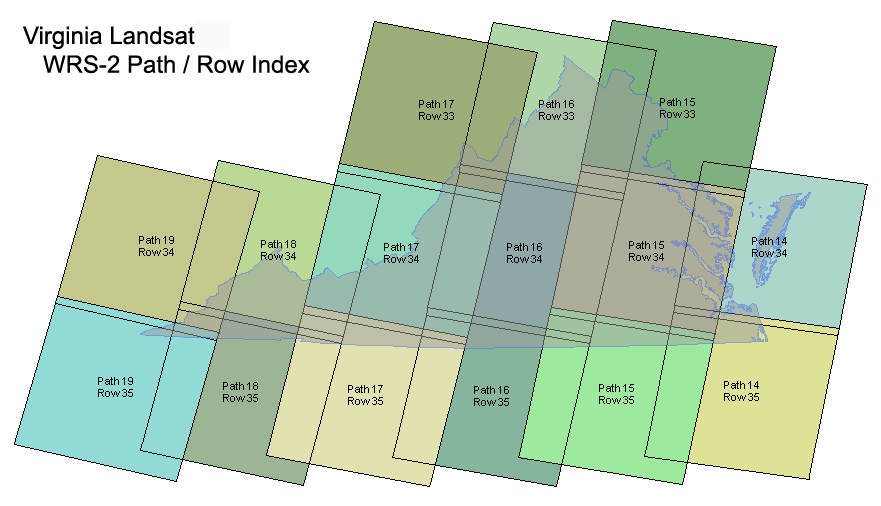
\includegraphics[scale=0.13]{images/covering/wrs.png}
  \caption{Landsat-8 grid covering (path,row) for Virginia ($USA$) }
\end{figure}
\end{frame}

\subsection{Image Georeferencement}
\begin{frame}
\tableofcontents[currentsubsection]
\end{frame}

\begin{frame}
Landsat-8 images are georeferenced : each pixel has (x,y) coordinates in a certain Projection Coordinates 
System (\begin{itshape}UTM Mercator\end{itshape})\\
\begin{columns}

\begin{column}{5cm}
\begin{figure}
  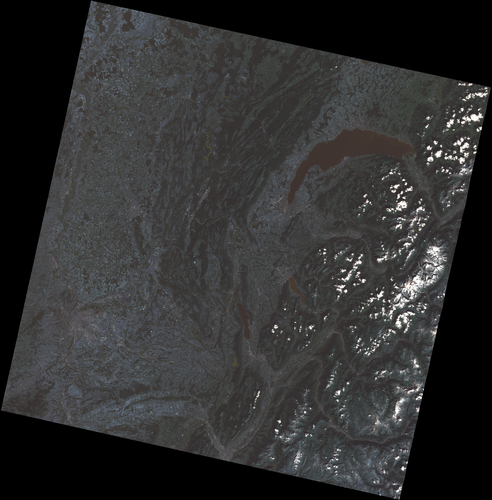
\includegraphics[scale=0.2]{images/georeferencing/Thonon_landsat.png}
  \caption{Landsat-8 grid covering (path,row) for Virginia ($USA$) }
\end{figure}
\end{column}

\begin{column}{5cm}
\begin{block}{coordinates}
 %\begin{itemize}
  %\item [upper left point] t\\
  %\item [upper right point] a\\
  %\item [bottom right point] x\\
  %\item [bottom left point] i\\
  %\end{itemize}
 \end{block}
\end{column}

\end{columns}

\end{frame}

\begin{frame}
Landast-8 georeferencing can be checked comparing with another georeferenced source like $IGN$ using a $SIG$ (open source $QGIS$).\\
\begin{columns}
 \begin{column}{3cm}
    \begin{figure}
        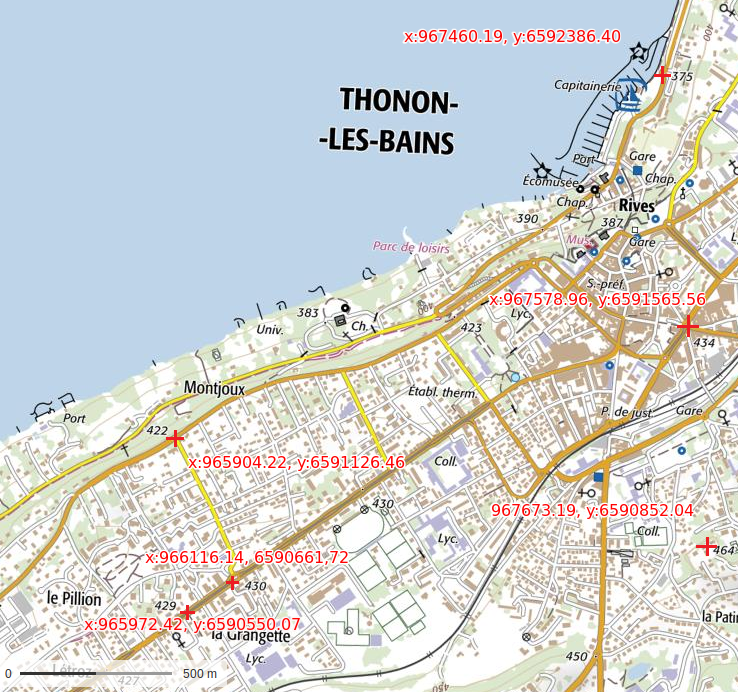
\includegraphics[scale=0.13]{images/georeferencing/ign-points-Thonon.png}
        \caption{IGN georeferenced image from $Lambert$ $93$ }
    \end{figure}
  \end{column}
 \begin{column}{2cm}
    \begin{figure}
        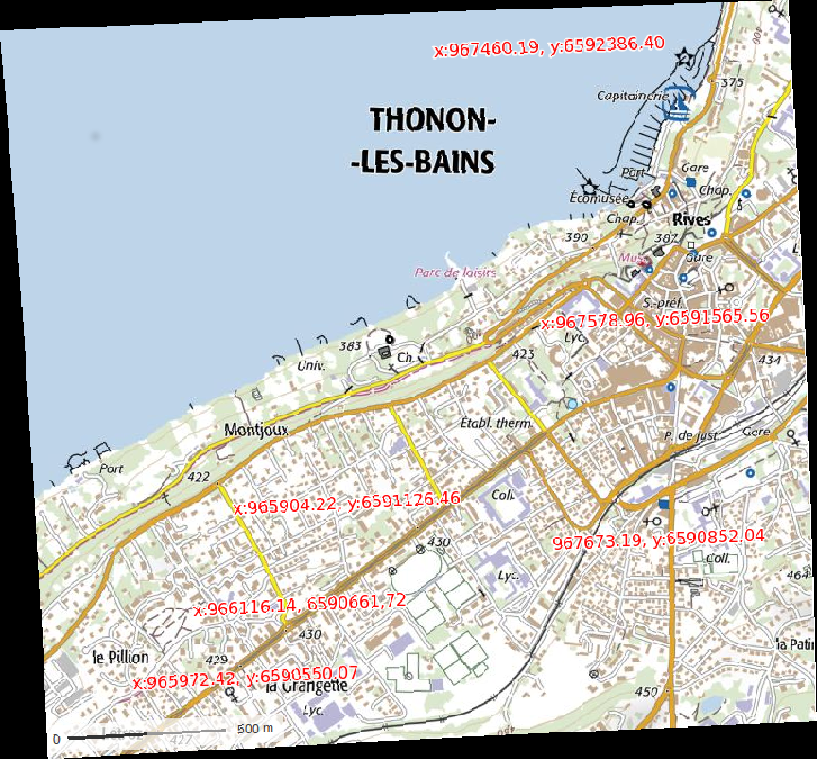
\includegraphics[scale=0.09]{images/georeferencing/qgis-resultat.png}
        \caption{IGN georeferenced image to $UTM$ $Mercator$}
    \end{figure}
  \end{column}
 \begin{column}{5cm}
    \begin{figure}
        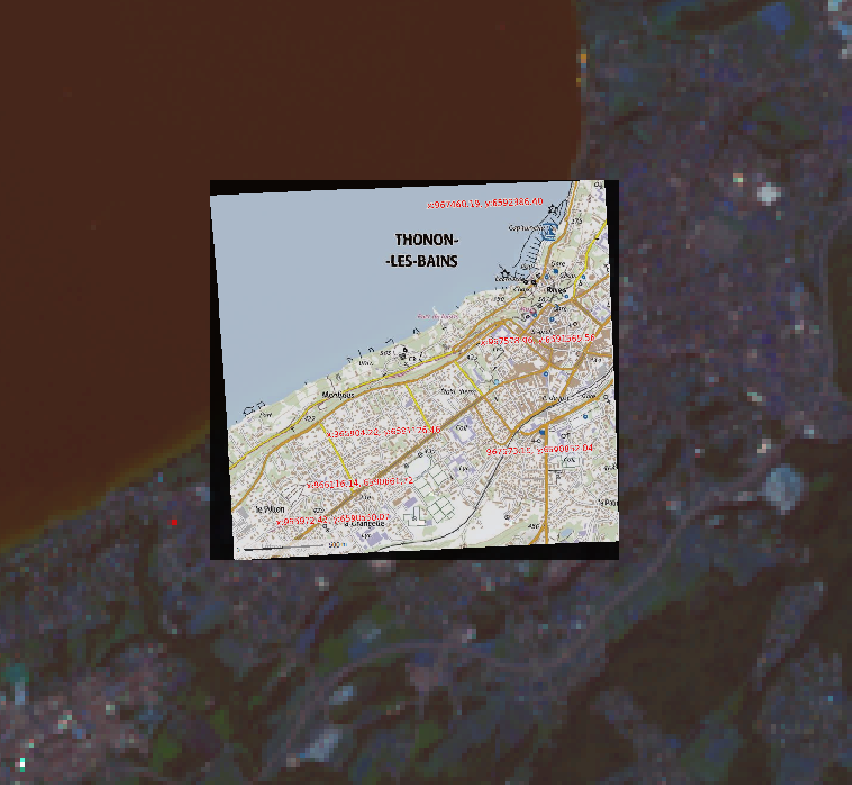
\includegraphics[scale=0.09]{images/georeferencing/qgis-superposition0.png}
        \caption{IGN georeferenced image ($UTM$ $Mercator$) superposed with Landsat-8 georeferenced image ($UTM$ $Mercator$) }
    \end{figure}
 \end{column}
\end{columns}
\end{frame}

\subsection{Importing images}
\begin{frame}
 
\end{frame}

\subsection{Image query}
\begin{frame}
 
\end{frame}

\subsection{Image bands}
\begin{frame}
 
\end{frame}

\section{Importing labels}
\begin{frame}
 
\end{frame}

\section{Vegetation index extraction}

\subsection{NDVI extraction}
\begin{frame}

\end{frame}

\subsection{NDVI evolution}
\begin{frame}

\end{frame}

\subsection{Data to Machine Learning}
\begin{frame}
 
\end{frame}

\section{Supervised Regression}
\begin{frame}

\end{frame}

\section{Supervised Classification}
\begin{frame}

\end{frame}

\end{document}
